\documentclass{beamer}

\usepackage{graphicx}
\usepackage{tikz-network}
\usepackage[table]{xcolor}

\title{Graph Theory}
\author{Melissa Carvajal, Carmen Hidalgo \& Josu\'e Soto}
\institute{Investigaci\'on de Operaciones}
\date{2025}

\begin{document}
\maketitle

\begin{frame}

\frametitle{Floyd's Algorithm}
This program consists of Floyd's algorithm to obtain the shortest path between any pair of nodes in a graph with weighted distances.
Floyd's algorithm compares the distance between any two given nodes and by passing through another city in between, if the result is less than the original then it chooses the shortest one. After contemplating all nodes in the graph, the graph is guaranteed to have all the shortest distances between any two nodes in the graph. These changes are recorded in another matrix called P that helps determine the shortest path between any two nodes.
\end{frame}



\begin{frame}
\frametitle{Robert W. Floyd (1936–2001)}
\begin{figure}

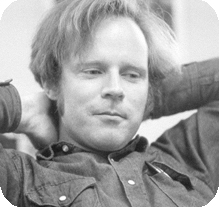
\includegraphics[width=0.25\textwidth]{floyd.jpg}
\caption{\label{fig:floyd}Robert Floyd}
\end{figure}
Robert Willoughby Floyd was a computer scientist that lived from 1936 to 2001. He made great advances in computer science and developed an algorithm to find the shortest paths between any two nodes for a directed graph. He was awarded a Turing Award in 1978.
\end{frame}


\begin{frame}
\frametitle{Initial Graph}
\begin{center}
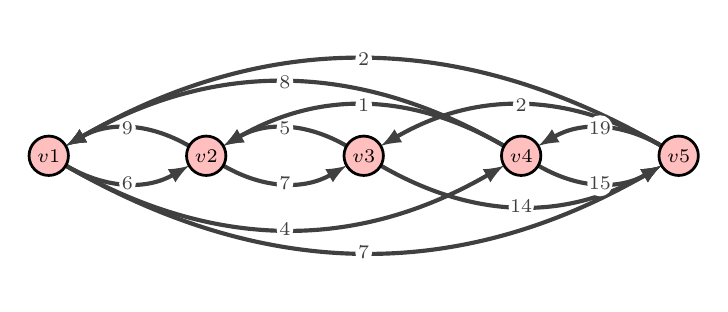
\begin{tikzpicture}
 \Vertex[x=0, y=0, color=pink, size=0.5, label=$v1$]{A}
 \Vertex[x=2, y=0, color=pink, size=0.5, label=$v2$]{B}
 \Vertex[x=4, y=0, color=pink, size=0.5, label=$v3$]{C}
 \Vertex[x=6, y=0, color=pink, size=0.5, label=$v4$]{D}
 \Vertex[x=8, y=0, color=pink, size=0.5, label=$v5$]{E}
 
 \Edge[bend=-30, label=$6$, Direct](A)(B) 
 \Edge[bend=-30, label=$4$, Direct](A)(D) 
 \Edge[bend=-30, label=$7$, Direct](A)(E) 
 \Edge[bend=-30, label=$9$, Direct](B)(A) 
 \Edge[bend=-30, label=$7$, Direct](B)(C) 
 \Edge[bend=-30, label=$5$, Direct](C)(B) 
 \Edge[bend=-30, label=$14$, Direct](C)(E) 
 \Edge[bend=-30, label=$8$, Direct](D)(A) 
 \Edge[bend=-30, label=$1$, Direct](D)(B) 
 \Edge[bend=-30, label=$15$, Direct](D)(E) 
 \Edge[bend=-30, label=$2$, Direct](E)(A) 
 \Edge[bend=-30, label=$2$, Direct](E)(C) 
 \Edge[bend=-30, label=$19$, Direct](E)(D)\end{tikzpicture}
\end{center}
\end{frame}



\begin{frame}
\frametitle{Table $D_{0}$}
\begin{center}
    \begin{tabular}{|c||c|c|c|c|c|}
        \hline
        \textbf{D} & \textbf{v1} & \textbf{v2} & \textbf{v3} & \textbf{v4} & \textbf{v5} \\
        \hline
        \hline
        \textbf{v1}& 0 & 6 & $\infty$ & 4 & 7 \\
        \hline
        \textbf{v2}& 9 & 0 & 7 & $\infty$ & $\infty$ \\
        \hline
        \textbf{v3}& $\infty$ & 5 & 0 & $\infty$ & 14 \\
        \hline
        \textbf{v4}& 8 & 1 & $\infty$ & 0 & 15 \\
        \hline
        \textbf{v5}& 2 & $\infty$ & 2 & 19 & 0 \\
        \hline
    \end{tabular}
\end{center}


\end{frame}





\begin{frame}
\frametitle{Table $P_{0}$}
\begin{center}
    \begin{tabular}{|c||c|c|c|c|c|}
        \hline
        \textbf{P} & \textbf{v1} & \textbf{v2} & \textbf{v3} & \textbf{v4} & \textbf{v5} \\
        \hline
        \hline
        \textbf{v1}& 0 & 0 & 0 & 0 & 0 \\
        \hline
        \textbf{v2}& 0 & 0 & 0 & 0 & 0 \\
        \hline
        \textbf{v3}& 0 & 0 & 0 & 0 & 0 \\
        \hline
        \textbf{v4}& 0 & 0 & 0 & 0 & 0 \\
        \hline
        \textbf{v5}& 0 & 0 & 0 & 0 & 0 \\
        \hline
    \end{tabular}
\end{center}


\end{frame}





\begin{frame}
\frametitle{Table $D_{1}$}
\begin{center}
    \begin{tabular}{|c||c|c|c|c|c|}
        \hline
        \textbf{D} & \textbf{v1} & \textbf{v2} & \textbf{v3} & \textbf{v4} & \textbf{v5} \\
        \hline
        \hline
        \textbf{v1}& 0 & 6 & $\infty$ & 4 & 7 \\
        \hline
        \textbf{v2}& 9 & 0 & 7 & \cellcolor[HTML]{D74894}$13$ & \cellcolor[HTML]{D74894}$16$ \\
        \hline
        \textbf{v3}& $\infty$ & 5 & 0 & $\infty$ & 14 \\
        \hline
        \textbf{v4}& 8 & 1 & $\infty$ & 0 & 15 \\
        \hline
        \textbf{v5}& 2 & \cellcolor[HTML]{D74894}$8$ & 2 & \cellcolor[HTML]{D74894}$6$ & 0 \\
        \hline
    \end{tabular}
\end{center}


\end{frame}





\begin{frame}
\frametitle{Table $P_{1}$}
\begin{center}
    \begin{tabular}{|c||c|c|c|c|c|}
        \hline
        \textbf{P} & \textbf{v1} & \textbf{v2} & \textbf{v3} & \textbf{v4} & \textbf{v5} \\
        \hline
        \hline
        \textbf{v1}& 0 & 0 & 0 & 0 & 0 \\
        \hline
        \textbf{v2}& 0 & 0 & 0 & \cellcolor[HTML]{D74894}$1$ & \cellcolor[HTML]{D74894}$1$ \\
        \hline
        \textbf{v3}& 0 & 0 & 0 & 0 & 0 \\
        \hline
        \textbf{v4}& 0 & 0 & 0 & 0 & 0 \\
        \hline
        \textbf{v5}& 0 & \cellcolor[HTML]{D74894}$1$ & 0 & \cellcolor[HTML]{D74894}$1$ & 0 \\
        \hline
    \end{tabular}
\end{center}


\end{frame}





\begin{frame}
\frametitle{Table $D_{2}$}
\begin{center}
    \begin{tabular}{|c||c|c|c|c|c|}
        \hline
        \textbf{D} & \textbf{v1} & \textbf{v2} & \textbf{v3} & \textbf{v4} & \textbf{v5} \\
        \hline
        \hline
        \textbf{v1}& 0 & 6 & \cellcolor[HTML]{D74894}$13$ & 4 & 7 \\
        \hline
        \textbf{v2}& 9 & 0 & 7 & 13 & 16 \\
        \hline
        \textbf{v3}& \cellcolor[HTML]{D74894}$14$ & 5 & 0 & \cellcolor[HTML]{D74894}$18$ & 14 \\
        \hline
        \textbf{v4}& 8 & 1 & \cellcolor[HTML]{D74894}$8$ & 0 & 15 \\
        \hline
        \textbf{v5}& 2 & 8 & 2 & 6 & 0 \\
        \hline
    \end{tabular}
\end{center}


\end{frame}





\begin{frame}
\frametitle{Table $P_{2}$}
\begin{center}
    \begin{tabular}{|c||c|c|c|c|c|}
        \hline
        \textbf{P} & \textbf{v1} & \textbf{v2} & \textbf{v3} & \textbf{v4} & \textbf{v5} \\
        \hline
        \hline
        \textbf{v1}& 0 & 0 & \cellcolor[HTML]{D74894}$2$ & 0 & 0 \\
        \hline
        \textbf{v2}& 0 & 0 & 0 & 1 & 1 \\
        \hline
        \textbf{v3}& \cellcolor[HTML]{D74894}$2$ & 0 & 0 & \cellcolor[HTML]{D74894}$2$ & 0 \\
        \hline
        \textbf{v4}& 0 & 0 & \cellcolor[HTML]{D74894}$2$ & 0 & 0 \\
        \hline
        \textbf{v5}& 0 & 1 & 0 & 1 & 0 \\
        \hline
    \end{tabular}
\end{center}


\end{frame}





\begin{frame}
\frametitle{Table $D_{3}$}
\begin{center}
    \begin{tabular}{|c||c|c|c|c|c|}
        \hline
        \textbf{D} & \textbf{v1} & \textbf{v2} & \textbf{v3} & \textbf{v4} & \textbf{v5} \\
        \hline
        \hline
        \textbf{v1}& 0 & 6 & 13 & 4 & 7 \\
        \hline
        \textbf{v2}& 9 & 0 & 7 & 13 & 16 \\
        \hline
        \textbf{v3}& 14 & 5 & 0 & 18 & 14 \\
        \hline
        \textbf{v4}& 8 & 1 & 8 & 0 & 15 \\
        \hline
        \textbf{v5}& 2 & \cellcolor[HTML]{D74894}$7$ & 2 & 6 & 0 \\
        \hline
    \end{tabular}
\end{center}


\end{frame}





\begin{frame}
\frametitle{Table $P_{3}$}
\begin{center}
    \begin{tabular}{|c||c|c|c|c|c|}
        \hline
        \textbf{P} & \textbf{v1} & \textbf{v2} & \textbf{v3} & \textbf{v4} & \textbf{v5} \\
        \hline
        \hline
        \textbf{v1}& 0 & 0 & 2 & 0 & 0 \\
        \hline
        \textbf{v2}& 0 & 0 & 0 & 1 & 1 \\
        \hline
        \textbf{v3}& 2 & 0 & 0 & 2 & 0 \\
        \hline
        \textbf{v4}& 0 & 0 & 2 & 0 & 0 \\
        \hline
        \textbf{v5}& 0 & \cellcolor[HTML]{D74894}$3$ & 0 & 1 & 0 \\
        \hline
    \end{tabular}
\end{center}


\end{frame}





\begin{frame}
\frametitle{Table $D_{4}$}
\begin{center}
    \begin{tabular}{|c||c|c|c|c|c|}
        \hline
        \textbf{D} & \textbf{v1} & \textbf{v2} & \textbf{v3} & \textbf{v4} & \textbf{v5} \\
        \hline
        \hline
        \textbf{v1}& 0 & \cellcolor[HTML]{D74894}$5$ & \cellcolor[HTML]{D74894}$12$ & 4 & 7 \\
        \hline
        \textbf{v2}& 9 & 0 & 7 & 13 & 16 \\
        \hline
        \textbf{v3}& 14 & 5 & 0 & 18 & 14 \\
        \hline
        \textbf{v4}& 8 & 1 & 8 & 0 & 15 \\
        \hline
        \textbf{v5}& 2 & 7 & 2 & 6 & 0 \\
        \hline
    \end{tabular}
\end{center}


\end{frame}





\begin{frame}
\frametitle{Table $P_{4}$}
\begin{center}
    \begin{tabular}{|c||c|c|c|c|c|}
        \hline
        \textbf{P} & \textbf{v1} & \textbf{v2} & \textbf{v3} & \textbf{v4} & \textbf{v5} \\
        \hline
        \hline
        \textbf{v1}& 0 & \cellcolor[HTML]{D74894}$4$ & \cellcolor[HTML]{D74894}$4$ & 0 & 0 \\
        \hline
        \textbf{v2}& 0 & 0 & 0 & 1 & 1 \\
        \hline
        \textbf{v3}& 2 & 0 & 0 & 2 & 0 \\
        \hline
        \textbf{v4}& 0 & 0 & 2 & 0 & 0 \\
        \hline
        \textbf{v5}& 0 & 3 & 0 & 1 & 0 \\
        \hline
    \end{tabular}
\end{center}


\end{frame}





\begin{frame}
\frametitle{Table $D_{5}$}
\begin{center}
    \begin{tabular}{|c||c|c|c|c|c|}
        \hline
        \textbf{D} & \textbf{v1} & \textbf{v2} & \textbf{v3} & \textbf{v4} & \textbf{v5} \\
        \hline
        \hline
        \textbf{v1}& 0 & 5 & \cellcolor[HTML]{D74894}$9$ & 4 & 7 \\
        \hline
        \textbf{v2}& 9 & 0 & 7 & 13 & 16 \\
        \hline
        \textbf{v3}& 14 & 5 & 0 & 18 & 14 \\
        \hline
        \textbf{v4}& 8 & 1 & 8 & 0 & 15 \\
        \hline
        \textbf{v5}& 2 & 7 & 2 & 6 & 0 \\
        \hline
    \end{tabular}
\end{center}


\end{frame}





\begin{frame}
\frametitle{Table $P_{5}$}
\begin{center}
    \begin{tabular}{|c||c|c|c|c|c|}
        \hline
        \textbf{P} & \textbf{v1} & \textbf{v2} & \textbf{v3} & \textbf{v4} & \textbf{v5} \\
        \hline
        \hline
        \textbf{v1}& 0 & 4 & \cellcolor[HTML]{D74894}$5$ & 0 & 0 \\
        \hline
        \textbf{v2}& 0 & 0 & 0 & 1 & 1 \\
        \hline
        \textbf{v3}& 2 & 0 & 0 & 2 & 0 \\
        \hline
        \textbf{v4}& 0 & 0 & 2 & 0 & 0 \\
        \hline
        \textbf{v5}& 0 & 3 & 0 & 1 & 0 \\
        \hline
    \end{tabular}
\end{center}


\end{frame}


\begin{frame}
\frametitle{Final Graph}
\begin{center}
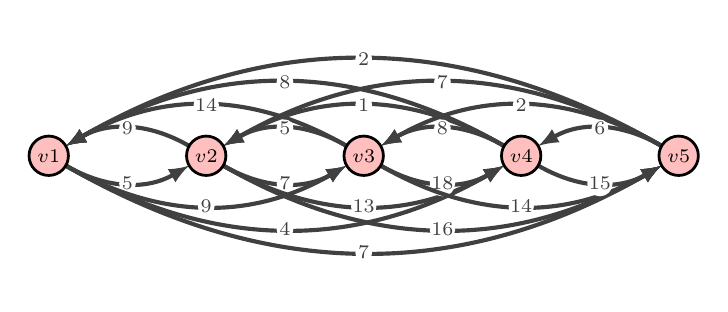
\begin{tikzpicture}
 \Vertex[x=0, y=0, color=pink, size=0.5, label=$v1$]{A}
 \Vertex[x=2, y=0, color=pink, size=0.5, label=$v2$]{B}
 \Vertex[x=4, y=0, color=pink, size=0.5, label=$v3$]{C}
 \Vertex[x=6, y=0, color=pink, size=0.5, label=$v4$]{D}
 \Vertex[x=8, y=0, color=pink, size=0.5, label=$v5$]{E}
 
 \Edge[bend=-30, label=$5$, Direct](A)(B) 
 \Edge[bend=-30, label=$9$, Direct](A)(C) 
 \Edge[bend=-30, label=$4$, Direct](A)(D) 
 \Edge[bend=-30, label=$7$, Direct](A)(E) 
 \Edge[bend=-30, label=$9$, Direct](B)(A) 
 \Edge[bend=-30, label=$7$, Direct](B)(C) 
 \Edge[bend=-30, label=$13$, Direct](B)(D) 
 \Edge[bend=-30, label=$16$, Direct](B)(E) 
 \Edge[bend=-30, label=$14$, Direct](C)(A) 
 \Edge[bend=-30, label=$5$, Direct](C)(B) 
 \Edge[bend=-30, label=$18$, Direct](C)(D) 
 \Edge[bend=-30, label=$14$, Direct](C)(E) 
 \Edge[bend=-30, label=$8$, Direct](D)(A) 
 \Edge[bend=-30, label=$1$, Direct](D)(B) 
 \Edge[bend=-30, label=$8$, Direct](D)(C) 
 \Edge[bend=-30, label=$15$, Direct](D)(E) 
 \Edge[bend=-30, label=$2$, Direct](E)(A) 
 \Edge[bend=-30, label=$7$, Direct](E)(B) 
 \Edge[bend=-30, label=$2$, Direct](E)(C) 
 \Edge[bend=-30, label=$6$, Direct](E)(D)\end{tikzpicture}
\end{center}
\end{frame}
\end{document}
